\section{Labels}\label{sec:labels}

\subsection{Overview}


Concurrent programs are a mix of control constructs ($\cseq,\parallel,+,\dots$)
and atomic actions $a$ that modify \emph{program state} $s$.
This is all that is visible to the programmer.



Our denotational UTP semantics
is inspired by that done for UTPP\cite{DBLP:conf/icfem/WoodcockH02},
itself based on a UTP theory of \emph{action systems}.
In UTPP a new state component, not visible in the program text,
was added: a set of labels ($ls$).
These labels are used to orchestrate the flow of control.
Given an atomic action $a$ that only knows about program state $s$,
we use notation $\catom a$ to describe a lifted version
of $a$ that takes account of the contents of the label-set $ls$.
In effect a lifted atomic state action is disabled until
a particular label is present in that set.
A disabled action does not modify the state any way
and simply monitors the label-set.
Once an action observes the presence/arrival of its label,
it then becomes active.
An active lifted action $\catom a$ atomically modifies the extended state as follows:
\begin{itemize}
  \item It makes the changes to $s$ as determined by its underlying action $a$.
  \item It removes the enabling label from the label-set.
  \item It adds in appropriate ``continuation'' labels to $ls$.
\end{itemize}
In \cite{DBLP:conf/icfem/WoodcockH02},
the language syntax required explicit (starting) labels
for every atomic state change action,
and these are used as lifted action enablers.
The continuation labels were taken to the the enabling labels
of whatever other actions occurred immediately after, in the program.
This means that the resulting semantics is not compositional.

The approach we adopt here is to adopt the notion of \emph{label generators}
to create the labels, so ensuring they are unique,
but in such a way as make the generation a compositional process.
In addition we explicitly associate two labels with every program construct:
one that marks the entry into the construct,
and another that indicates the exit.
In our UTP theory we will introduce two static observation variables,
$in$ and $out$ to record respectively the entry and exit labels
for a given construct.


\subsection{Label Generation}

We want to have a way to associate unique labels
with every atomic action, including those added to manage flow of control,
in a compositional manner.
We start by assuming that we have types for labels,
and label generators:
\RLEQNS{
   l &\in& Lbl
\\ g &\in& Gen
}
We have two distinct things we can do with label generators:
\begin{enumerate}
  \item
   Use it then generate a label,
   in which case we also need to get a transformed generator
   that is guaranteed to never produce the label just generated.
   \RLEQNS{
     new &:&  Gen \fun (Lbl \times Gen)
     & \elabel{new-sig}
   }
  \item
   Split generators into two new generators,
   each of which will produce disjoint sets of labels.
   \RLEQNS{
     split &:& Gen \fun (Gen \times Gen)
     & \elabel{split-sig}
   }
\end{enumerate}
Given $new$ and $split$ above, we can defined a function $labs$ that
returns all the labels produced by a generator,
and express our label uniqueness guarantees.
Assuming that $ (l,g') = new(g)$ and $(g_1,g_2) = split(g)$
we get:
\RLEQNS{
   labs &:& Gen \fun \power Lbl & \elabel{labs-sig}
\\ labs(g)
   &\defs&
   \setof l \cup labs(g')
   \cup
   labs(g_1) \cup labs(g_2) &\ecite{labs-def}
\\ l &\notin& labs(g') &\ecite{new-disj}
\\ labs(g_1) \cap labs(g_2) &=&  \emptyset & \ecite{split-disj}
}

Given the notion of label generators as just described,
we are faced with two problems.
The first is that the notation is quite clumsy:
For example in the semantics to be presented below,
we will need the following generator expression:
$
\pi_2(new(\pi_2(new(\pi_2(split(g))))))
$,
where $\pi_i$ projects out the $i$th element of a pair.
The second is that our definitions above are axiomatic,
and we need to demonstrate some form of model that satisfies
the above laws (\ecite{new-disj},\ecite{split-disj}).
Ideally this should also avoid some sort of global check for uniqueness,
to ensure compositionality of the resulting semantics.

Fortunately,
it turns out there is a shorthand notation that dramatically shortens
generator and label expressions,
while also providing a compositional model that satisfies the laws above.

\subsubsection{Generator Notation}

The idea is to realise that we really have four functions of interest:
\RLEQNS{
   \pi_1 \circ new &:& Gen \fun Lbl
\\ \pi_2 \circ new &:& Gen \fun Gen
\\ \pi_1 \circ split &:& Gen \fun Gen
\\ \pi_2 \circ split &:& Gen \fun Gen
}
For the first one, we shall define a prefix operator $\ell : Gen \fun Lbl$
and render its generator argument as a subscript:
\RLEQNS{
  \ell_g &\defs& \pi_1(new(g)) & \elabel{ell-def}
}

For the other three, we turn them into single-character postfix operators,
themselves being rendered as subscripts:
\RLEQNS{
   \g{:} &\defs& \pi_2 \circ new & \elabel{new-:-def}
\\ \g1   &\defs& \pi_1 \circ split & \elabel{split-1-def}
\\ \g2   &\defs& \pi_2 \circ split & \elabel{split-2-def}
}
We then introduce a notation of generator and label expressions
with the following syntax:
\RLEQNS{
   G \in Gen &::=&  g     & \mbox{the ``root'' generator}
\\           &\mid& G_{:} & \mbox{resulting generator after label produced}
\\           &\mid& G_1   & \mbox{first generator after generator split}
\\           &\mid& G_2   & \mbox{second generator after generator split}
\\ L \in Lbl &::=& \ell_G & \mbox{label produced by generator}
}
Note that our generator expression language has only one variable, $g$,
which denotes the ``root'' generator.
We say the  ``root'' generator because this notion is local to a
particular context, and we can relativise things by replacing $g$
by an appropriate $G$ expression.
We can now revisit our definition of $labs$ and our disjointness rules
with the new notation:
\RLEQNS{
   labs &:& Gen \fun \power Lbl
\\ labs(G) &=& \setof{\ell_G} \cup labs(G_{:}) \cup labs(G_1) \cup labs(G_2)
  &\elabel{labs-def}
\\ \ell_G &\notin& labs(G_{:})
   &\elabel{new-disj}
\\ \emptyset &=& labs(G_1) \cap labs(G_2)
  &\elabel{split-disj}
}
The our complicated example shown earlier:
\[
\pi_2(new(\pi_2(new(\pi_2(split(g))))))
\]
now reduces to
\[
  \g{2::}
\]
If we generate a label with this generator,
then we simplify from
\[
\pi_1(new(\pi_2(new(\pi_2(new(\pi_2(split(g))))))))
\]
to
\[
  \ell_{g2::}
\]

We can also introduce a graphical way to visualise
generators that proves useful as a way to understand
the semantic definitions that occur later on,
as shown in Fig. \ref{fig:new-and-split}
\begin{figure}%
  \centering
  \parbox{1.2in}{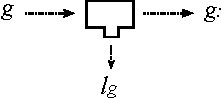
\includegraphics{images/new-label}}%
  \qquad\qquad
  \begin{minipage}{1.2in}%
    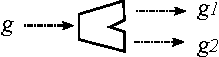
\includegraphics{images/split-gen}
  \end{minipage}%
  \caption{Graphical renderings of $new$ (left) and $split$ (right)}%
  \label{fig:new-and-split}%
\end{figure}



\subsubsection{Model for $new$ and $split$}

The conceptually simplest model of such generators
is one where labels produced are simply the strings of $:$, $1$ and $2$
that designate how the generator was produced from the original root.
For full clarity we show the model here using the full notation.
Both generators and labels are now represented as sequences of the three symbols
$:$, $1$ and $2$.
\RLEQNS{
  s \in LblSym &=& \setof{\texttt{:},\texttt{1},\texttt{2}}
\\ g \in GenSym &=& LblSym^*
\\ l \in Label &=& LblSym^*
\\ new(g) &\defs&  (g,g \cat \seqof{\texttt{:}})
\\ split(g) &\defs&  (g \cat \seqof{\texttt{1}},g \cat \seqof{\texttt{2}})
}
With this model we also get the following law:
For any generator expression $G$,
the following four sets are mutually disjoint:
\[
  \setof{\ell_G}
  \quad
  labs(G_{:})
  \quad
  labs(G_1)
  \quad
  labs(G_2)
  \qquad
  \elabel{labs-fully-disjoint}
\]
This is stronger than we require, but this is not a problem.
We also get three very significant benefits from this model/notation:
\begin{enumerate}
  \item
    It is very easy to decide if two generator expressions
    denote the same label---they do if and only if the expressions are the
    same, which in shorthand terms means the label sequences are the same.
  \item
    It is almost as easy to decide if two generator expressions produce
    disjoint labels.
    This occurs if and only if neither of the sequences of postfix operators
    involved are a prefix of the other.
    Or put differently, a generator's labels are a subset of another's
    iff its postfix sequence extends that of the other generator:
    \RLEQNS{
       labs(\g{\rho}) \subseteq labs(\g{\varrho}) &\equiv& \varrho \leq \rho
       & \elabel{prefix-lab-subset}
    }
    where $\leq$ is the sequence prefix relation.
  \item
    We refer to $g$ as the ``root'' in double quotes,
    because $g$ is not privileged in any way.
    If we substitute a different expression $G$ for $g$
    in the semantics of a construct,
    the behaviour is unchanged.
    In effect $g$ is like a ``base address'',
    with all the labels generated from $g$ being relative to it,
    and replacing $g$ by $G$ simply relocates it and the labels it generates.
    This is the basic mechanism used to construct the semantics
    of all the composite constructs in the language.
\end{enumerate}


\subsection{Label-Set Invariants}

The semantics we propose here depends on the careful management
of when specific labels are, or are not,
present in the global label-set $ls$.
We are looking at a situation where the semantics of any construct
requires associating unique labels with its entry and exit points,
as well as having a label generator provided for use with any sub-components
it might have.

So, from the perspective of any well-program $P$,
we have the following three (static) observation variables.
\RLEQNS{
   in, out &:& Lbl
\\ g &:& Gen
}
Key to the success of this semantics is a collection of label-set invariants
which characterise proper label-set contents,
which are preserved by all label-set manipulations performed
by our semantic definitions.

\subsubsection{Disjoint Labels (DL)}\label{sssec:disjoint-labels}

The first invariant we have is simply one that asserts,
for every construct, that $in$, $out$ and the labels of $g$
are all different
\footnote{The theory can be developed using only $g$ as a static observation,
and letting $\ell_g$ and $\ell_{g:}$ play the role of $in$ and $out$
respectively, in which case Disjoint Labels is automatically satisfied.
However, while this results in an entirely equivalent theory,
it is notationally much more obscure
with definitions and results that are harder to interpret and check.
}%
\RLEQNS{
   in \neq out &\land& \setof{in,out} \cap labs(g) = \emptyset
   & \ecite{Disjoint-Labels}
}



\subsubsection{Label Exclusivity (LE)}\label{sssec:label-exclusivity}

In addition to Disjoint Labels above,
which merely ensures distinctness of labels themselves,
we also need stronger invariants regarding which labels can, or cannot,
occur in the global label set at any one time.
There is not one such Label Exclusivity invariant,
but rather we have that each language construct defines it own
variation, in order to ensure that flow of control is correctly managed.

There is a general version of the invariant, as follows:
\RLEQNS{
   &&
   in \in  ls \implies (\setof{out} \cup labs(g))\cap ls = \emptyset
\\ &\land&
   (labs(g) \cap  ls \neq \emptyset) \implies \setof{in,out}\cap ls = \emptyset
\\ &\land&
   out \in ls \implies (\setof{in} \cup labs(g))\cap ls = \emptyset
   & \ecite{Exclusive-Labels}
}

We also more specific invariants, specific to each composite language construct.
We start with one of the simplest,
namely that used by sequential composition.
It asserts that any point in time,
only one of $in$, $\ell_g$ or $out$ can be present in $ls$:
\RLEQNS{
   &&
   in \in  ls \implies \setof{\ell_g,out}\cap ls = \emptyset
\\ &\land&
   \setof{\ell_g} \subseteq ls \implies \setof{in,out}\cap ls = \emptyset
\\ &\land&
   out \in ls \implies \setof{in,\ell_g}\cap ls = \emptyset
}
The most complex example is that for parallel composition.
Here we have four labels in addition to $in$ and $out$,
namely $\ell_{g1}$, $\ell_{g1:}$, $\ell_{g2}$, and $\ell_{g2:}$.
They should not occupy $ls$ at the same time as either $in $ or $out$,
but we also have that only one of the pair $(\ell_{g1},\ell_{g1:})$
can be present at the same time,
and the same must hold  for $(\ell_{g2},\ell_{g2:})$.
\RLEQNS{
   &&
   in \in ls
   \implies
   \setof{\ell_{g1},\ell_{g1:},\ell_{g2},\ell_{g2:},out}\cap ls = \emptyset
\\ &\land&
   \ell_{g1} \in ls \implies \setof{in,\ell_{g1:},out}\cap ls = \emptyset
\\ &\land&
   \ell_{g1:} \in ls \implies \setof{in,\ell_{g1},out}\cap ls = \emptyset
\\ &\land&
   \ell_{g2} \in ls \implies \setof{in,\ell_{g2:},out}\cap ls = \emptyset
\\ &\land&
   \ell_{g2:} \in ls \implies \setof{in,\ell_{g2},out}\cap ls = \emptyset
\\ &\land&
   out \in ls
   \implies
   \setof{in, \ell_{g1},\ell_{g1:},\ell_{g2},\ell_{g2:}}\cap ls = \emptyset
}
The precise motivation for these will be explained when the relevant
construct semantics are being described later.
For now we simply observe,
that these invariants are quite bulky and complex.



\subsubsection{Label-Set Invariant Notation}

First we shorten $labs(g)$ to just $g$ when this is clear from context,
i.e., a label-set, rather than a generator, is expected.

The Disjoint Labels invariant basically asserts
that a number of sets of labels are mutually disjoint.
We use the following shorthand, where the $L_i$ are label-sets,
\RLEQNS{
   \setof{L_1|L_2|\dots|L_n}
   &\defs&
   \forall_{i,j \in 1\dots n}
    @
    i \neq j \implies L_i \cap L_j = \emptyset
\\ \multicolumn{3}{c}{\elabel{short-disj-lbl}}
}
So we have an alternative definition of the Disjoint Labels invariant:
\RLEQNS{
 && \setof{in|g|out} & \elabel{Disjoint-Labels}
}

In a similar vein, we use a similar shorthand notation
for the Label Exclusivity invariants.
We use a shorthand,
whose easy cases can be formulated as follows:
\RLEQNS{
   ~[L_1|L_2|\dots|L_n]
   &\defs&
   \forall_{i,j \in 1\dots n}
    @
    i \neq j \implies
     ( L_i \cap ls \neq \emptyset \implies L_j \cap ls = \emptyset )
\\ \multicolumn{3}{c}{\elabel{short-lbl-exclusive}}
}
So the sequential composition Label Exclusivity invariant
is simply: $[in|\ell_g|out]$.
What needs to be kept in mind regarding this shorthand notation
is that $ls$ is mentioned under the hood,
and it is really all about what can be present in the global label-set
at any instant in time.

For parallel composition, we a little more complexity.
In shorthand it is expressed as
\[
   [in|(\ell_{g1}|\ell_{g1:}),(\ell_{g2}|\ell_{g2:})|out].
\]
It asserts at the top-level that $ls$
may contain only $in$, only $out$,
or only labels in $\ell_{g1},\ell_{g1:},\ell_{g2},\ell_{g2:}$.
In addition however, $\ell_{g1}$ and $\ell_{g1:}$ cannot occur together
and neither can $\ell_{g2}$ and $\ell_{g2:}$.

A more detailed and formal description of this way of describing
these invariants, in terms of an different abstract notation,
is presented in \S\ref{ssec:exclusive-lsat}.

\subsubsection{Properties of DL and LE}

Consider the following two generic examples:
\begin{enumerate}
  \item
    $DL_n = [L_1|L_2|\dots|L_n]$
    asserts that each $L_i$ is disjoint from any other.
  \item
    $LE_n = \{L_1|L_2|\dots|L_n\}$
    asserts that if elements one $L_i$ are in $ls$,
    then no elements from the others are.
\end{enumerate}

The ordering in either invariant is immaterial.
If $\rho$ is a permutation over $\setof{1\dots n}$ then
\RLEQNS{
   \{L_1|L_2|\dots|L_n\} &=& \{L_{\rho1}|L_{\rho2}|\dots|L_{\rho n}\}
   & \elabel{DL-perm}
\\ ~[L_1|L_2|\dots|L_n] &=& [L_{\rho1}|L_{\rho2}|\dots|L_{\rho n}]
   & \elabel{LE-perm}
}
Both invariants imply shorter versions of themselves:
\RLEQNS{
   \{\dots|L_{i-1}|L_i|L_{i+1}\dots\} &\implies& \{\dots|L_{i-1}|L_{i+1}\dots\}
   & \elabel{DL-drop}
\\ ~[\dots|L_{i-1}|L_i|L_{i+1}\dots] &\implies& [\dots|L_{i-1}|L_{i+1}\dots]
   & \elabel{LE-drop}
}
Both invariants imply versions with smaller sets:
\RLEQNS{
   S_i \subseteq L_i \land \{L_1|\dots|L_n\}
   &\implies& \{S_1|\dots|S_n\}
   & \elabel{DL-subset}
\\ S_i \subseteq L_i \land [L_1|\dots|L_n]
   &\implies& [S_1|\dots|S_n]
   & \elabel{DL-subset}
}
A key property shared by all LE invariants,
is that they are trivially satisfied by $ls = \emptyset$,
or if $ls$ only contains labels not mentioned in the invariant.
\RLEQNS{
   scope(LE_n) &\defs& L_1 \cup L_2 \cup \dots \cup L_n
\\ (ls = ls \setminus scope(LE_n)) &\implies& LE_n = \true
    & \elabel{LE-out-of-scope}
\\ ls = \emptyset &\implies& LE_n = \true
    & \elabel{LE-trivial}
}
There is no simple relationship between $DL_n$ and $LE_n$.
It is possible for one to be true when the other is false.
\begin{description}
  \item[DL true, LE false]
    $L_1 \cap L_2 = \emptyset \quad\land\quad (L_1 \cup L_2) \subseteq ls$.
  \item[DL false, LE true]
    $L_1 = L_2 \quad\land\quad L_1 \cap ls = \emptyset$
\end{description}
